\documentclass[10pt]{jarticle}
\usepackage{float}
\usepackage{adrobo_abst}
\usepackage[dvipdfmx]{graphicx}
\usepackage{amssymb,amsmath}
\usepackage{bm}
\usepackage[superscript]{cite}
\usepackage{enumerate}
\usepackage{url}
%\usepackage[absolute]{textpos}

\renewcommand\citeform[1]{(#1)}

\begin{document}
    
    \makeatletter
    \doctype{2023年度卒業論文概要}
    \title{論文の作成について}{(副題がある場合は括弧でくくる)}
    \etitle{Making Research Paper}{($\bigcirc\bigcirc\bigcirc$)}
    
    \author{20Cxxxx\hspace{.5zw}未来太郎}
    \eauthor{Taro MIRAI}
    
    \makeatother
    
    \abstract{When preparing the manuscript, read and observe carefully this sample as well as the instruction manual for the manuscript of the Transaction of Japan Society of Mechanical Engineers. This sample was prepared using MS-word. Character size of the English title is 14 pts of Times New Roman as well as sub-title. The name is 12 pts. The address of the first author and the abstract is 10 pts of Times New Roman. Character spacing of the abstract is narrowed by 0.2 pts preferably.}
    
    \keywords{Mechanical Engineering, Keywords List}
    
    \maketitle
    
    \supervisor{指導教員:未来次郎 准教授}
    
    \section{緒\hspace{2zw}言}%===========================
    
    本稿では,研究概要作成に関する主な原稿体裁をまとめた.
    
    本文には,半角かな文字は使用せず,文章の区切りには全角の読点(,)と句点(.)を用いる.
    
    \section{記号・単位の書き方}%===========================
    \begin{table}[!h]
        \begin{tabular}{lcl}
            $L$ & : & 長さ [m] \\
            $t$ & : & 時間 [s] \\
            $x$ & : & 流れ方向の座標 [m] \\
            $\alpha$ & : & 熱伝達率 [$\mathrm{W/(m^2\cdot K)}$] \\
            $Re$ & : & レイノルズ数 \\
            $\bm{R}$ & : & 回転行列 \\
            $\bm{t}$ & : & 並進ベクトル \\
        \end{tabular}
    \end{table}
    
    量記号はイタリック体,単位記号はローマン体,無次元数はイタリック体で書く.
    数学記号・単位記号及び量記号は,半角英数字を使用する.単位は,SI単位を使用し,4~MPa のように書く.
    
    分野によって作法は異なるが,わかりやすさの観点から行列の表記は大文字のイタリック体・ボールド体を推奨し,ベクトルの表記は小文字のイタリック体・ボールド体を推奨する.
    
    \section{見出しの書き方}%===========================
    
    論文の章立ては.章・節・項である.章見出しはゴシック体で記述し,2行分をとって行の中ほどに書く.
    18字以上は3行分を必要とするが,見出しが不必要に長くなるのは推奨されない.
    
    \subsection{節の書き方}
    
    項の見出しもゴシック体で記述し,本文は見出し後に改行をせずに,直後に2文字分の空白を空けてから書き始める.
    
    \begin{center}
        \begin{figure}[!b]
            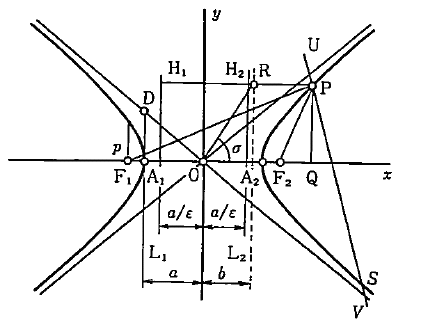
\includegraphics[width=0.45\textwidth]{./fig/sample.png}
            \caption{Sample of clear figure}
            \label{fig:sample-fig}
        \end{figure}
    \end{center}
    
    \section{図及び写真・表の作成に関して}%===========================
    \begin{enumerate}
        \setlength{\parskip}{0cm} % 段落間
        \setlength{\itemsep}{0cm} % 項目間
        \item 本文中では,\reffig{sample-fig},\reftab{sample-tab}のように日本語で書く.写真は,図として扱う.
        \item 番号・説明(キャプション)などは,図・写真についてはその下に,表についてはその上に書く.
        \item 本文と,図・表の間は1行以上の空白を空けて,見やすくする.
        \item 図中・表中の説明及びキャプションはすべて英語で書く(最初の文字は大文字とする).
        \item 図及び表がl列(片側)に収まらない場合2列(両側)にまたがって書くことができる. 
        \item 図及び表の横に空白ができても,その空白部には本文を記入してはならない.
    \end{enumerate}
    
    \begin{table}[t]
        \caption{Sample of expression of values}
        \label{tab:sample-tab}
        \begin{center}
            \vskip 1zh
            \begin{tabular}{|c|c|}
                \hline
                Recommend & Not recommend \\ \hline
                $0.357$ & $.357$ \\ \hline
                $3.141\ 6$ & $3.141,6$ \\ \hline
                $3.141\ 6 \times 2.5$ & $3.141\ 6 \cdot 2.5$ \\ \hline
            \end{tabular}
        \end{center}
    \end{table}
    
    \section{数式の書き方}%===========================
    
    式番号は,式と同じ行に右寄せして( )の中に書く.また,本文で式を引用するときは,\refeqn{sample-eq1}のように書く.
    \begin{equation}
        \gamma(t) = \frac{ji}{N} \label{eq:sample-eq1}
    \end{equation}
    \begin{equation}
    \bar{C}(t)=\frac{1}{N}\sum_{i=1}^{N}C_i(t) \label{eq:sample-eq2}
    \end{equation}
    
    %\begin{table}[!b] \notag
    %\begin{minipage}{\textwidth}
    %\begin{tabular*}{\textwidth}{@{\extracolsep{\fill}}lr}
    %{\footnotesize
    %$\displaystyle 
    %u^*_{i,j} = u^n_{i,j} - \Delta t \left\{u^n_{i,j}\frac{u^n_{i+1,j} - u^n_{i-1,j}}{2\Delta x} + v^n_{i,j}\frac{u^n_{i,j+1} - u^n_{i,j-1}}{2\Delta y} + \frac{1}{Re}\left(\frac{u^n_{i+1,j} - 2u^n_{i,j} + u^n_{i-1,j}}{(\Delta x)^2} + \frac{u^n_{i,j+1} - 2u^n_{i,j} + u^n_{i,j-1}}{(\Delta y)^2}\right) \right\}
    %$}
    %& $\inlineTag\label{eq:long-eq} $
    %\end{tabular*}
    %\end{minipage}
    %\end{table}
    
    式を書くときは,2文字分空白を空ける.
    また,必要行数分を必ず使うようにして書く.
    3行必要とする式を2行につめて書いたり,2行に分かれる式を1行に収めたりしない.
    なお,本文と式,式相互間は1行以上の空白を空けて,見やすくする.
    ポイント数は本文に準じるものとするが,添え字等が小さく読みにくくなるときは適宜拡大する.
    
    %式はなるべく片側に書くことが望ましいが,両側にまたがる場合は,読む順序に混乱を生じないように,そのページの式の上,または下の本文全部を両方にまたがるように書かなければならない.
    %本見本では\refeqn{long-eq}のようにページの最上段もしくは最下段に配置している場合は,上記のような混乱は生じ得ないので以下の文章は2段組で続けることができる.
    %ただし,所望の位置に表示されない,文字が重なるなどレイアウト上の多くの問題が生じるため,極めて推奨しない.
    
    \section{引用文献の書き方}%===========================
    本文中の引用箇所には,右肩に小括弧をつけて,通し番号を付ける.例えば,文献\cite{工大2005}や,文献\cite{Shibutani2004, Handbook1979, Kikuchi2017, Adrobo2019}のようにする.
    
    引用文献は,英文で記述されているもの(文献\cite{Shibutani2004}など)は英文で書き,本文末尾に引用順にまとめて書く.専門的な書籍(文献\cite{Handbook1979}など)についても引用しても良い.
    Web上の資料を引用する場合,例えばオンラインジャーナルなどの場合は文献\cite{Kikuchi2017}のように,webページの場合は文献\cite{Adrobo2019}のように,それぞれ参考文献として記載して引用する.この時,URLとともに参照日を記載すること.ただし,webページの場合は個人の技術ブログなどのように第3者による十分な審査が行われていないものの引用は行ってはいけない.公的な機関が発行しているページであっても,その永続性の問題から必要最小限に留めることを推奨する.
        
    \section{結\hspace{2zw}言}%===========================
    このスタイルファイル「adrobo\_abst.sty」は,千葉工業大学 未来ロボティクス学科の卒業研究概要として公式に提出可能なように,学科で配布するwordテンプレートとレイアウトなどの体裁を合わせたものである.
    ただし,絶対的な出来上がりのレベルを保証するものではないため,執筆を進める上で不具合などが生じた場合は,直ちに製作者に通知をすることが望まれる.
    また,使用者によるスタイルファイルの微調整などに関しては,自己責任の範囲において自由に行って良い.
    
    \vspace{5truemm}
    {\footnotesize
        \begin{thebibliography}{99}
            
            \bibitem{工大2005}
            工大太郎: ``ロボットのしくみ'', 
            日本機械学会論文誌A, 
            Vol.~108, No.~1034 (2005), pp.~1--2.
            
            \bibitem{Shibutani2004}
            Y. Shibutani: ``Heinrich's Law Resulted Pattern Dynamics --Part2--'',
            Proceedings of the 79th Kansai Branch Regular Meeting of the Japan Society of Mechanical Engineers,  
            No.~04--05 (2004), pp.~205--206.
            
            \bibitem{Handbook1979}
            The Japan Society of Mechanical Engineers ed.: ``JSME Date Handbook: Heat Transfer'', 
            (1979), p.~123, The Japan Society of Mechanical Engineers.
            
            \bibitem{Kikuchi2017}
            K. Kikuchi, M. Miura, K. Shibata, J. Yamamura: ``Soft Landing Condition for Stair-climbing Robot with Hopping Mechanism'', 
            Journal of JSDE, Vol.~53, No.~8 (2018), pp.~605--614, \url{https://doi.org/10.14953/jjsde.2017.2774}.
            
            \bibitem{Adrobo2019}
            千葉工業大学 未来ロボティクス学科 学科概要: 
            \url{http://www.robotics.it-chiba.ac.jp/ja/subject/index.html}, 
            (参照日 2023年1月29日). 
            
        \end{thebibliography}
    }
    \normalsize
    
\end{document}
